
\chapter{Methodology}

\label{Chapter5:Methodology} 
%----------------------------------------------------------------------------------------
%	SECTION 1
%----------------------------------------------------------------------------------------

In this chapter we will discuss the entire work flow and the methods used in this study. Starting from the different model architecture used. We used two two main archetecture and with some configurations to answer our research questions. Also we will be discussing how the structural dataset was created and some pre processing applied in order to investigate on research question.


\section{System Overview}
We approached this problem of depth map estimation from monocular images to give end to end solution as much as possible using two CNN. As we discussed in the section \ref{Chapeter1:Topic_Description} our main focus was (a) to deliver a robust method and (b) regeneration of dead pixels or holes for better reconstruction of images. 

First, in order to deliver a robust network we first investigated and propose a simple model architecture and test against the existing. Our existing model is a simple U-Net style architecture - also can be categorized as encoder-decoder style of architecture. The reason for this model is to see if a simple network can learn the structural dependencies with respect to its depth. Knowing that the depth images are very much are highly structural dependent we wanted to see how well a network can learn without any prior knowledge. This motivated us to use an existing model to evaluate against the proposed model.We found out the our model performs relatively poor. We used the pre-trained weights of encoder and retrained the decoder layers with new structure dataset. And the results of this transfer leaning makes it more efficient. Hence we have 2 models, a simple U-Net with de-convolutional layers we call it as approach 1  (\textbf{A1}) and another model proposed by Alhashim et. al. \cite{Alhashim2018} and applied transfer learning approach we call it as approach 2 (\textbf{A2}) and \textbf{A2} become the main contribution for good results compared with U-Net approach model. 

Secondly, we wanted to investigate if a model can learn the holes generated from the SLB sensor. In our literature study we where unable to find previous work which was focused to make the network learn the holes and regenerated. The most common and widely used method was to either in paint the holes using neighboring pixel \cite{silberman11indoor} or some other methods where used. We approached this problem by saving the holes and map all the invalid holes to zero value instead of finding neighboring pixel which was used in NYU dataset. We trained \textbf{A2} model in two different fashion. One by mapping the holes to a zero value we call it as \textbf{A2-Holes} and another we find the neighboring pixels and we call this approach as \textbf{A2-NoHoles}. Note that, \textbf{A2-Holes} method might need some proprocessing as we will will discuss more in the results section \ref{Chapter6:Results}.

Therefore, we have two model \textbf{A1} and \textbf{A2} for validating the proposed model and effects of structural Characteristic. Further more \textbf{A2} model where retrained with two different modified input features for investigating on regeneration of holes. This gives us two more configuration of \textbf{A2} modelnamely \textbf{A2\_Holes} and \textbf{A2\_NoHoles}. 








\subsection{Approach 1 (A1) - U Net Style Network}
U-Net (\textbf{A1}) architecture as shown in Fig \ref{fig:A1-U-NetArchetecture} is built upon simple idea of using de-convolution layer  \footnote{not to be confused with the nomenclature, there are various names for de-convolution such as up-sampling layers or transposed convolution layer used by tensorflow and keras (\url{www.tensorflow.org/})} for up scaling the learnt feature and regeneration of depth maps. Hence the decoder block comprises of transposed 2D convolution layers which have the same dimension as the kernal size of encoder block. This means number of layers in encoder and decoder are the sample that's why the name U-Net. We use \textbf{A1} architecture since its easy to configure and understand how the up sample of network can be done. We \nadacn{Some more spec later}

\begin{figure}[t]
    \centering
    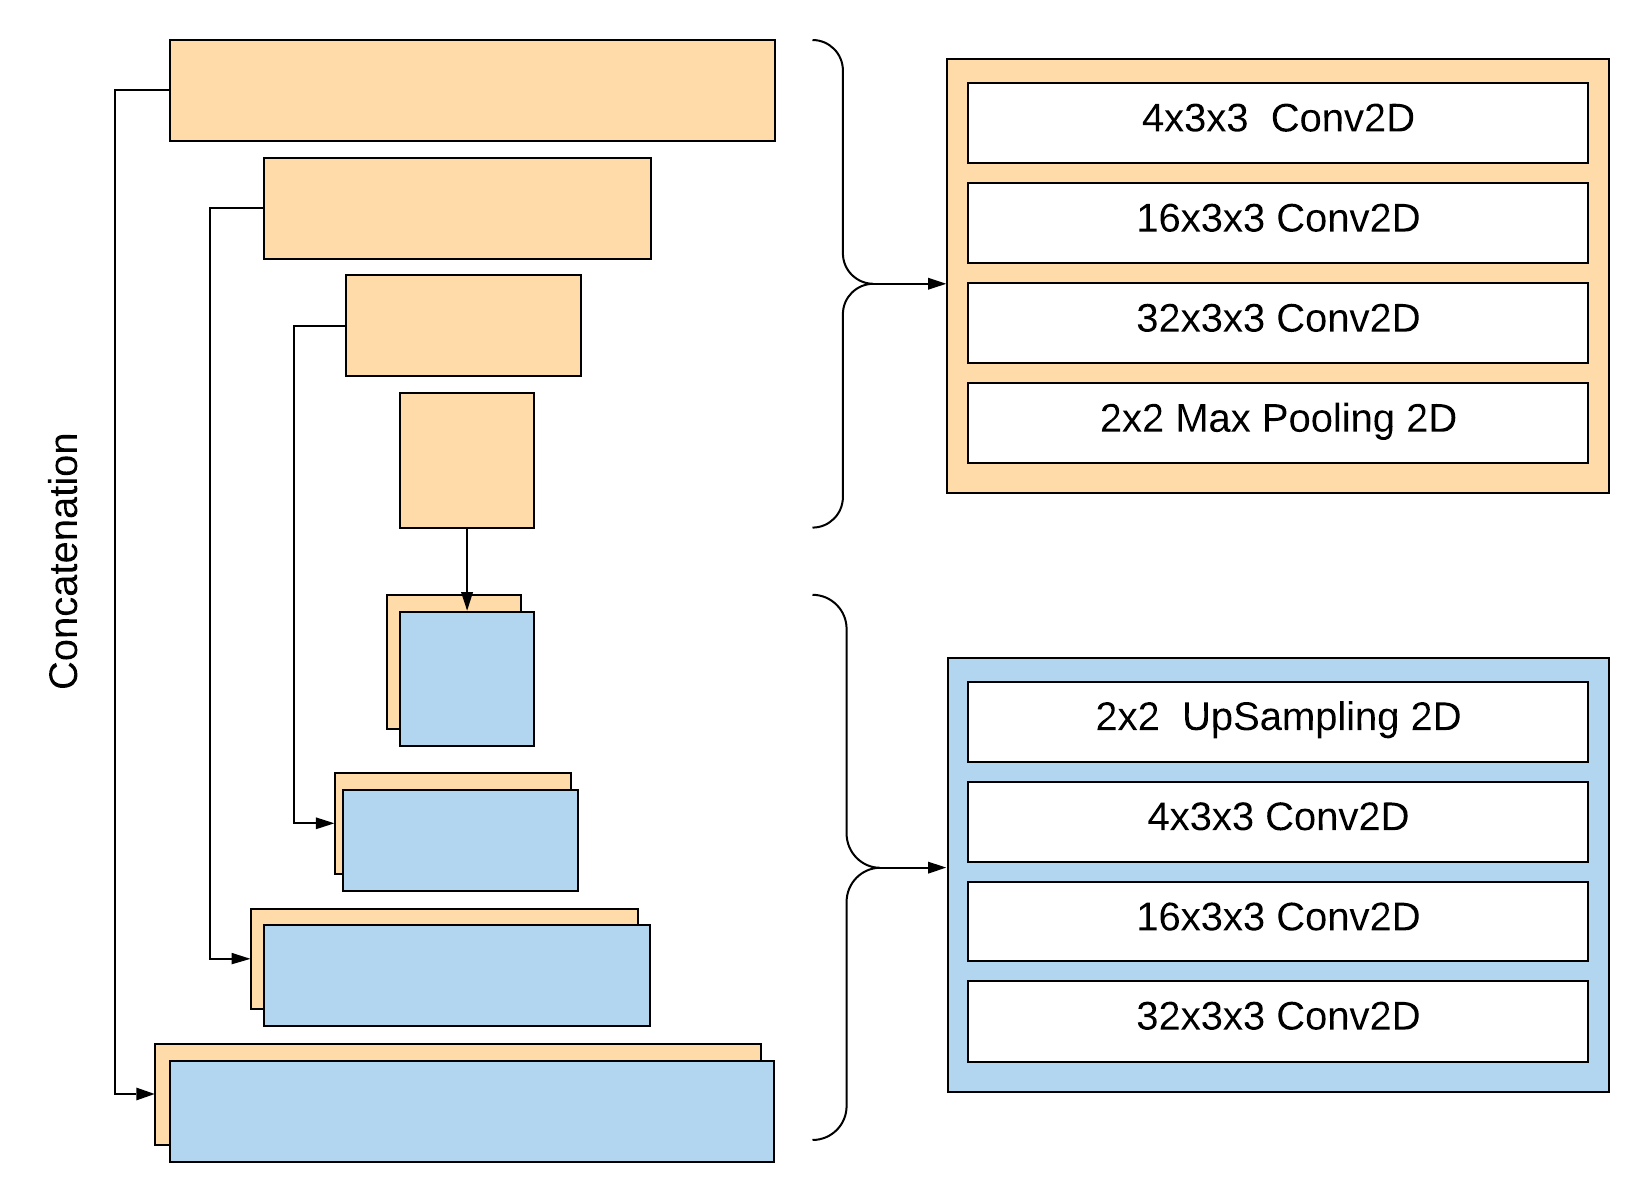
\includegraphics[width = 14cm, height = 9cm]{Figures/A1.png}
    \caption{U-Net architecture (\textbf{A1}). The arrow mark shows the concatenation of the higher level learnt feature from encoder to the upsamplng decoder part.}
    \label{fig:A1-U-NetArchetecture}
\end{figure}{}


\subsection{Approach 2 (A2) - DenseNet backbone}

Fig. \ref{fig:A1-U-NetArchetecture} shows an overview of our encoder-decoder network for depth estimation model proposed by Alhashim et. al. \cite{Alhashim2018}. The input RGB image is fed to the DenseNet-169 \cite{huang2017densely} network which is pretrained on ImageNet \cite{deng2009imagenet}. The output from the DenseNet block is then fed to a successive series of up-sampling layers.The decoder part is trained on the 120,000 images of NYU v2 depth dataset.  We have two option in order to reconstruct the final depth map at half the input resolution or at full resolution, this can be achived just by adding one more bi-linear upsampling layer at the end by the factor of 2 which gives us the resolution of $480 \times 640$.  For all the experiment we only used half resolution for ease of use and fast training.  Also the decoder does not contain any Batch Normalization or other advanced sub multi task layers as seen in the recent state-of-the-art methods in section \ref{Chapter3:RelatedWork_NNModel}. Backbone DenseNet architecture is designed in a feed forward fashion within a dense block or in other words such a a way that each layer is directly connected to every other layer. There are two types of DenseNet one for smaller images and another for lager images which is called DenseNetImageNet. 

We use this model and use transfer learning and train on Structure dataset which is described in the section \ref{}

\begin{figure}[h]
    \centering
    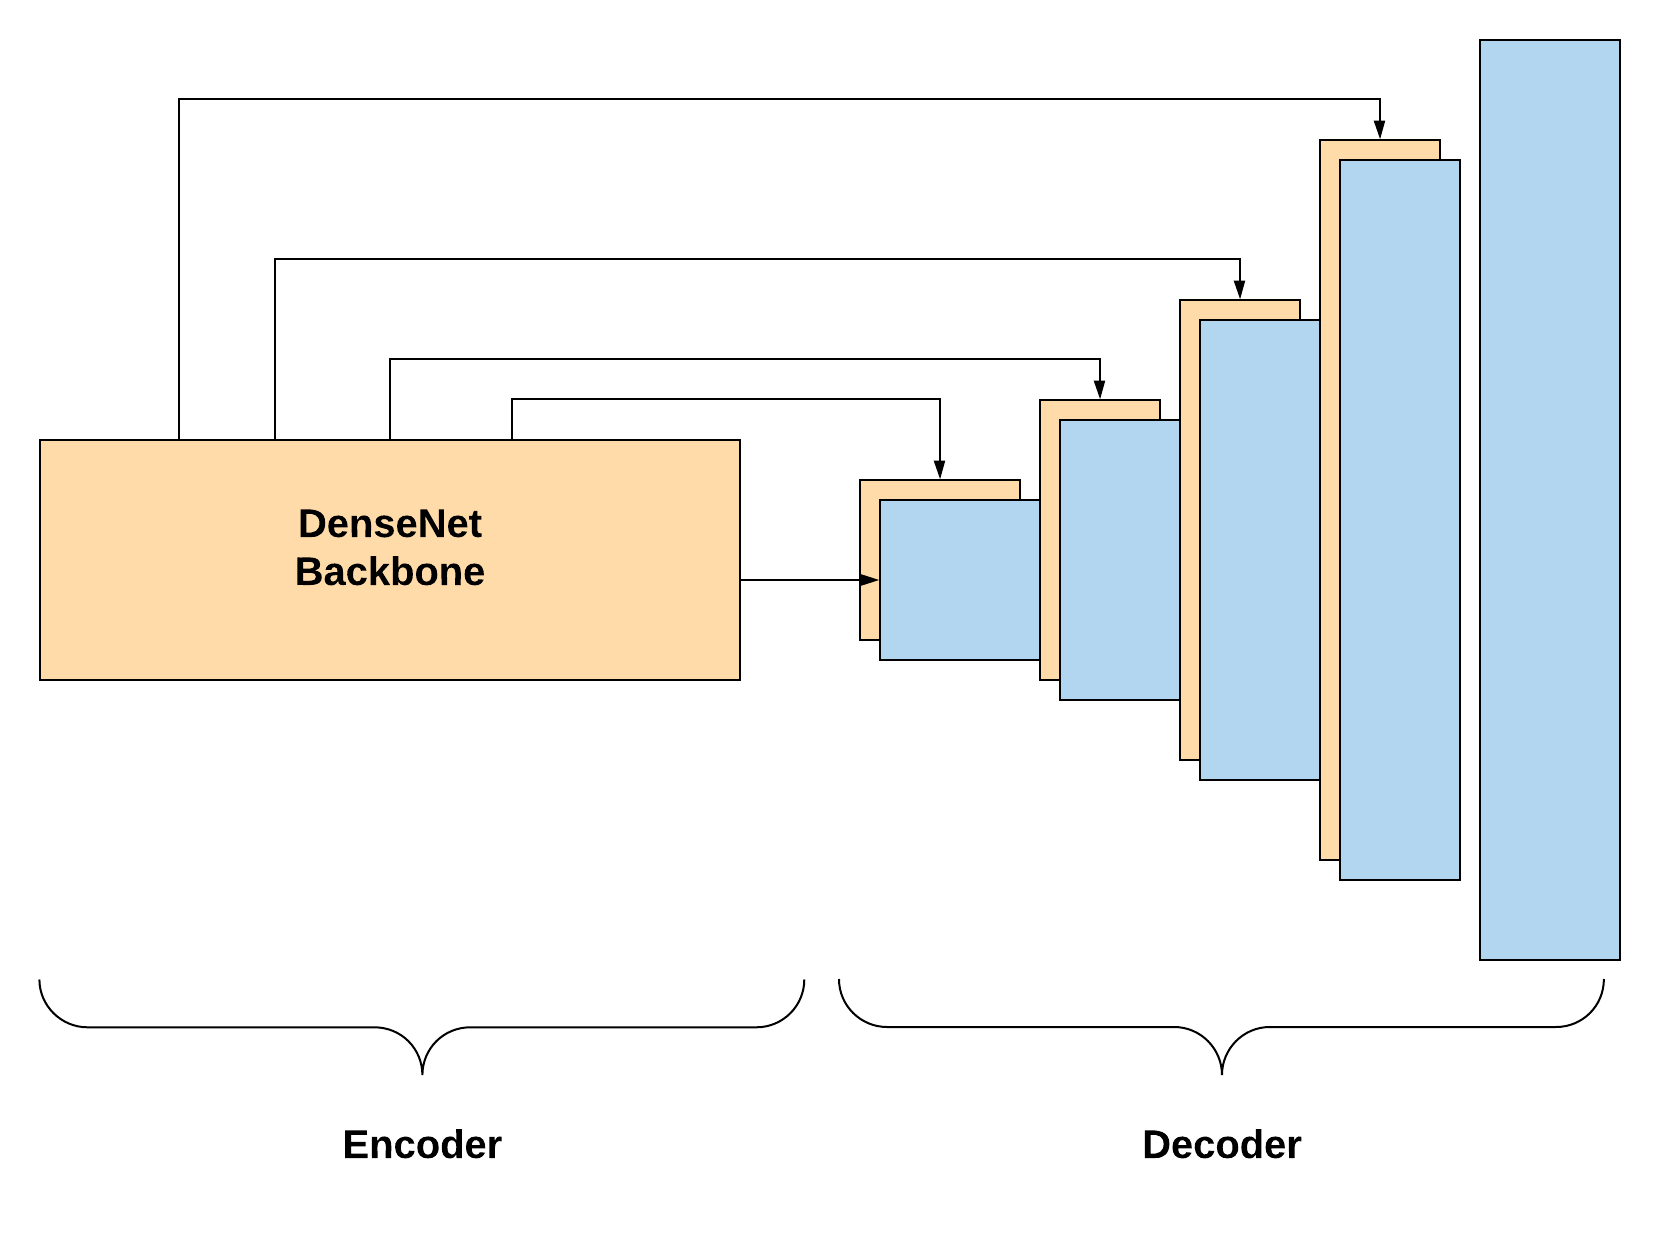
\includegraphics[width = 14cm,  height = 8.5cm]{Figures/A2.png}
    \caption{DenseNet}
    \label{fig:A2-DenseNet-arch}
\end{figure}{}







\section{Schedule and Milestones}
1 page: Provide a GANTT diagram based on week
